\chapter{Desenvolvimento}\label{cap_2_Fundamentaçao}

Neste capítulo, será discutido, inicialmente, uma visão geral do circuito completo e como seus componentes se comportam em conjunto para gerar um jogo de checagem de senha.

Após isso, detalhes de cada componente do circuito serão discutidos, além de como foi construído componentes maiores a partir de componentes mais basicos.

\section{O Circuito Completo}

%Estes quem?(segunda linha)
Neste circuito, visto na Figura \ref{fig:2.1}, tem-se os inputs dos botões entrando diretamente no \emph{Chave Led Buzzer}, descrito em 2.11. Estas chaves ligaram diretamente nos LEDs para indicar quais bits do hexadecimal de entrada estão ativos.

\begin{figure}[H]
	\centering
	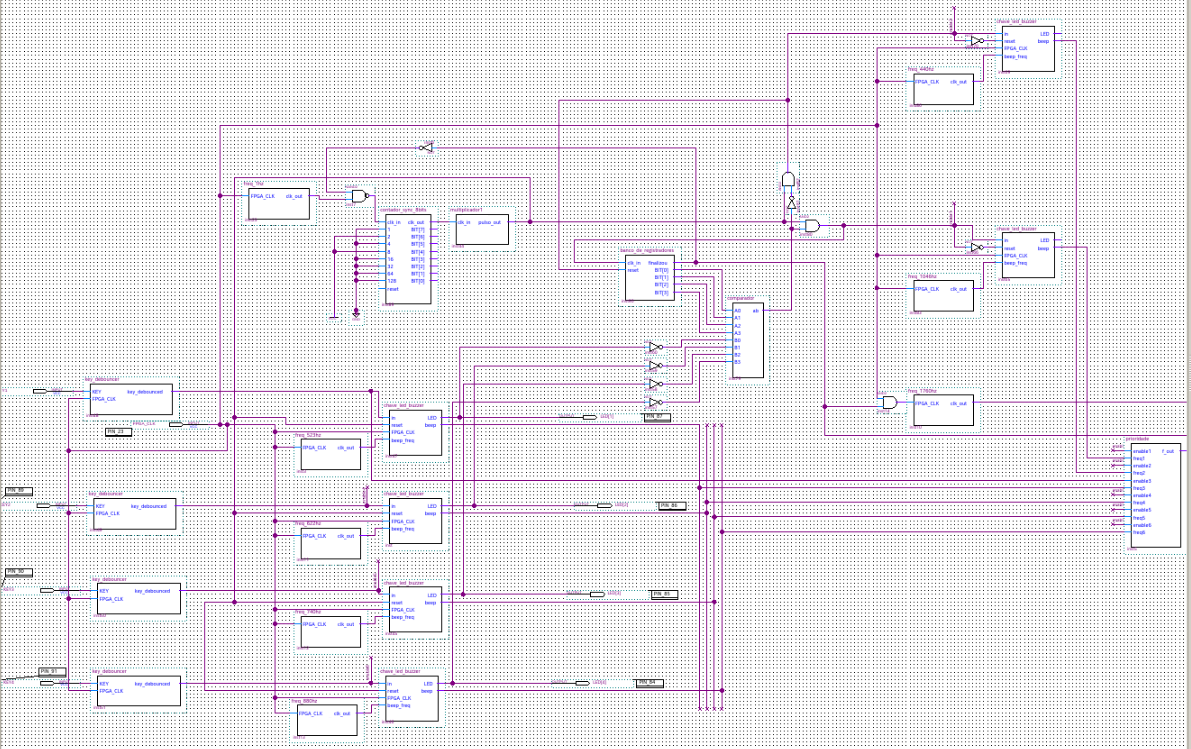
\includegraphics[width=1\columnwidth]{FIGURAS/cap_2/projeto.png}
	\caption{Representação esquemática do projeto completo.}
        \label{fig:2.1}
\end{figure}


Estes bits serão levados até o comparador. Lá, eles serão comparados com os bits que estão saindo do banco de registrador.

Simultaneamente, tem-se um clock com frequência de $1Hz$ sendo inserido em um contador módulo 10. Sua saída será transformada em pulso. Essa transformação é feita para poder-se ter um rising edge tanto na subida, quanto na descida do clock.

Este pulso será levado de volta pros \emph{Chave Led Buzzer} para dar reset neles, e permitir ao usuário a inserção do próximo dígito.

Estes pulsos também seguiram e bifurcaram em dois caminhos, dependendo do estado atual do comparador. Se o comparador confirmar que os dígitos estão corretos com os do hexadecimal de senha atual, um clock será dado no banco de registradores para pular pro próximo dígito, e uma frequência aguda é emitida no buzzer. Essa frequência dará mute nas frequências vindas dos botões.

Se o comparador afirmar que o dígito estava errado, o banco de comparadores é resetado e retorna-se ao primeiro hexadecimal.

Caso o registrador estore sua contagem, conclui-se que o último dígito da senha foi inserido corretamente, desconecta-se o clock de entrada do contador, da-se mute em todas frequências vindas dos botões e ativa-se uma frequência aguda para confirmar que o programa foi concluído.

Todas as frequências, exceto a de finalização do programa, estão em um sistema de prioridade descrito em 2.9, para impedir interferências.



\section{Flip-Flops}

Foi utilizado dois tipos de flip-flops no projeto, o tipo \emph{t} e o tipo \emph{d}.

Ambos têm entrada clear e preset, que quando estão, ambas, em nível lógico alto (1,1), não afetam a saída Q dos flip-flops.

Quando uma delas está em nível lógico baixo e a outra em nível lógico alto, elas tomam precedência sobre as entradas do flip-flop. A saída será definida como 1 se preset estiver em nível lógico baixo, ou 0, se o clear estiver em nível lógico baixo.

É um estado proibido ambos, clear e preset, estarem em nível lógico baixo (0,0).

\subsection{Tipo \emph{t}}

Na Figura \ref{fig:2.2} pode-se observar a representação do flip-flop tipo \emph{t}.

\begin{figure}[H]
	\centering
	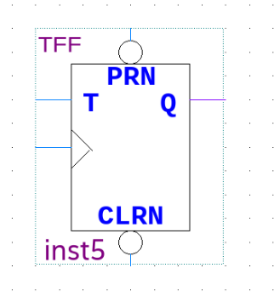
\includegraphics[width=0.3\columnwidth]{FIGURAS/cap_2/tff.png}
	\caption{Representação do flip-flop tipo t.}
        \label{fig:2.2}
\end{figure}

Neste flip-flop, a entrada \emph{T} define se a saída será invertida ou não quando houver uma subida (rising\_edge) do clock.

Este flip-flop foi utilizado extensivamente no modo inversor, ou seja com o \emph{T} em nível lógico alto.

\subsection{Tipo \emph{d}}

Na Figura \ref{fig:2.3} pode-se observar a representação do flip-flop tipo \emph{d}.

\begin{figure}[H]
	\centering
	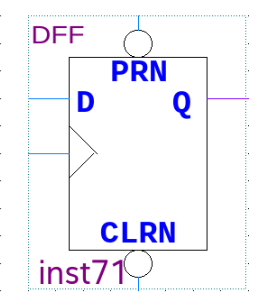
\includegraphics[width=0.3\columnwidth]{FIGURAS/cap_2/dff.png}
	\caption{Representação do flip-flop tipo d.}
        \label{fig:2.3}
\end{figure}

O flip-flop \emph{d}, passa o valor da entrada para a saída quando há uma subida (rising\_edge) no nível lógico do clock.

Ele foi utilizado como buffer de informação no tipo de conexão \emph{Q->D} e como inversor (similar ao tipo \emph{t}) quando \emph{NOT Q -> D}.

\section{Divisores}

Foi criado divisores de clock para controlar as mudanças de frequência do circuito. E também para estabilizar pulsos em clocks.

\subsection{Divisor1}

Na Figura \ref{fig:2.4} é apresentado o Divisor1.

\begin{figure}[H]
	\centering
	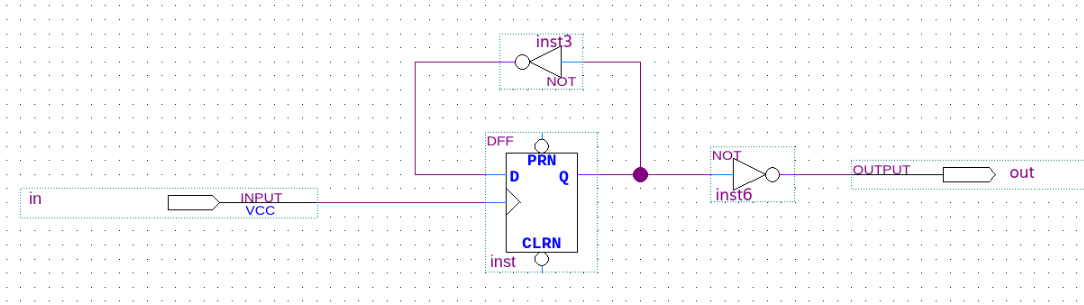
\includegraphics[width=1\columnwidth]{FIGURAS/cap_2/divisor1.png}
	\caption{Representação do Divisor1, que divide o clock pela metade.}
        \label{fig:2.4}
\end{figure}

Ele fará uma divisão de clock, de maneira decrescente utilizando um flip-flop do tipo \emph{d} na configuração inversora.

%Essa frase ficou certa?
Foi utilizado o modo decrescente, pois este era um requerimento do projeto para o controle do tempo do buzzer.

\subsection{Divisor8}

Neste, tem-se 8 Divisor1 em série, como pode ser visto na Figura \ref{fig:2.5}. Ele foi feito para dividir o clock em $2^8$.

\begin{figure}[H]
	\centering
	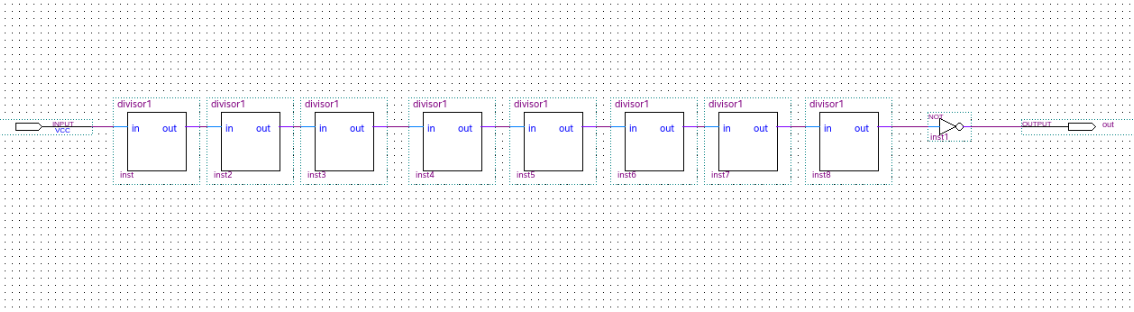
\includegraphics[width=1\columnwidth]{FIGURAS/cap_2/divisor8.png}
	\caption{Representacao do Divisor8, que divide o clock por $2^8$.}
        \label{fig:2.5}
\end{figure}

Ele foi utilizado para simplificar o diagrama de blocos quando precisa-se  dividir o clock por valores grandes.



\subsection{Divisor16}

Neste, tem-se 2 Divisor8 em série, como pode ser visto na Figura \ref{fig:2.6}. Ele foi feito para dividir o clock em $2^{16}$.

\begin{figure}[H]
	\centering
	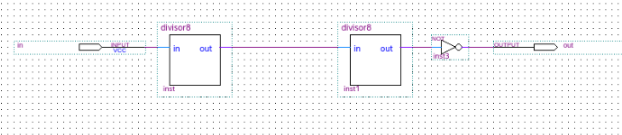
\includegraphics[width=1\columnwidth]{FIGURAS/cap_2/divisor16.png}
	\caption{Representacao do Divisor8, que divide o clock por $2^{16}$.}
        \label{fig:2.6}
\end{figure}


Ele também foi utilizdo para simplificar o diagrama de blocos quando precisa-se dividir o clock por valores grandes.



\section{Contadores}

Foi utlizado contadores como divisores precisos de clock, quando for requerido dividir esse clock por algo que não seja potência de $2$.

Foi criado um contador de 8 bits autoral para dividir as frequências do buzzer e foi utilizado o LPM Counter para fazer a divisão precisa do clock de 1Hz.


Ter utilizado o LPM Counter para ambos foi uma possibilidade, mas foi preferido criar o contador autoral para melhor entender o funcionamento de divisões de clock.

\subsection{Contador síncrono de 8 bits}

Aqui, na Figura \ref{fig:2.7} vê-se a "entrada" do contador de 8 bits.

\begin{figure}[H]
	\centering
	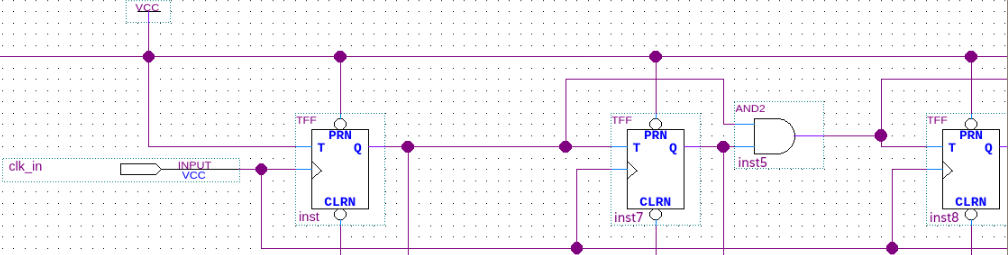
\includegraphics[width=1\columnwidth]{FIGURAS/cap_2/contador_8bits.png}
	\caption{Representação de parte do contador de 8 bits.}
        \label{fig:2.7}
\end{figure}



Quando ocorre uma subida de nível lógico (rising\_edge) do clock, todos flip-flops se acionam. E a inversão da saída de cada um ocorre de acordo com o estado atual da sua porta \emph{T}.

A porta \emph{T} do primeiro flip-flop da série sempre está ativa. Enquanto cada porta \emph{T} subsequente só estará em nível lógico alto quando a saída \emph{Q} do anterior estiver em nível alto lógico.

Ou seja, cada saída \emph{Q} inverterá a cada $2 ^ {sua\_posicao}$ clocks.

Aqui, na Figura \ref{fig:2.8} vê-se como foi escolhido quando resetar o contador. Ou seja, quando ele atingir seu \emph{Módulo}.

\begin{figure}[H]
	\centering
	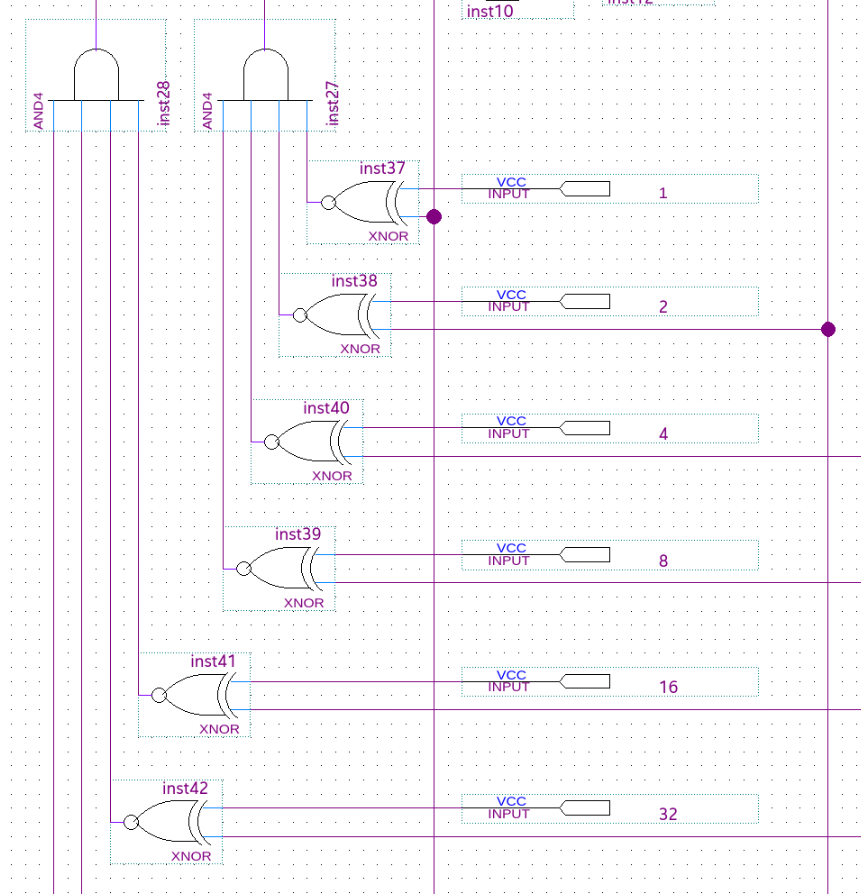
\includegraphics[width=1\columnwidth]{FIGURAS/cap_2/contador_8bits_reset.png}
	\caption{Representação da seleção de números para reset.}
        \label{fig:2.8}
\end{figure}



As saídas \emph{Q} são comparadas com inputs de entrada escolhidas pelo desenvolvedor do hardware. Quando a contagem atingir o valor pré-definido pelo desenvolvedor, passa-se um nível lógico baixo (falling\_edge) para os resets dos flip-flops do contador, forçando-o a retornar todos os valores para 0 e, consequentemente, as saídas \emph{Q} deixam de ser iguais aos inputs. Isso faz com que o reset retorne pro seu estado padrão de nível lógico alto.

Aqui, na Figura \ref{fig:2.9} vê-se que quando há a descida do nível lógico dos resets, ou seja, quando atinge-se o módulo e reinicia-se o contador, força-se uma subida no nível lógico do clock out. Isso ocorre  para indicar que houve um estouro na contagem.

\begin{figure}[H]
	\centering
	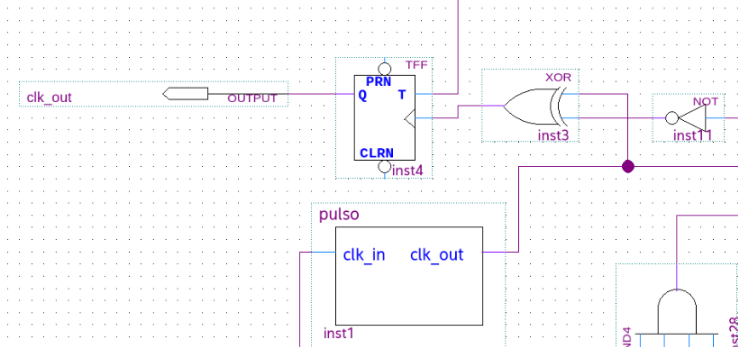
\includegraphics[width=1\columnwidth]{FIGURAS/cap_2/contador_8bits_clockout.png}
	\caption{Representação do clock out do contador de 8 bits.}
        \label{fig:2.9}
\end{figure}



Ele está em XOR com o pulso do input de reset do contador. Isso, porque quando utiliza-se o input reset, quer-se apenas reiniciar o contador, mas não enviar que houve um estouro da contagem.


\subsection{LPM Counter e Frequencia de 1Hz}

%O módulo era pra ser esse?
Neste, como pode ser observado na Figura \ref{fig:2.10}, foi definido o sentido da contagem, no caso crescente (UP), o módulo, $2.5E7$ e a quantidade de bits necessária, que no caso seria $Log_2(2.5E7) = 25$.

\begin{figure}[H]
	\centering
	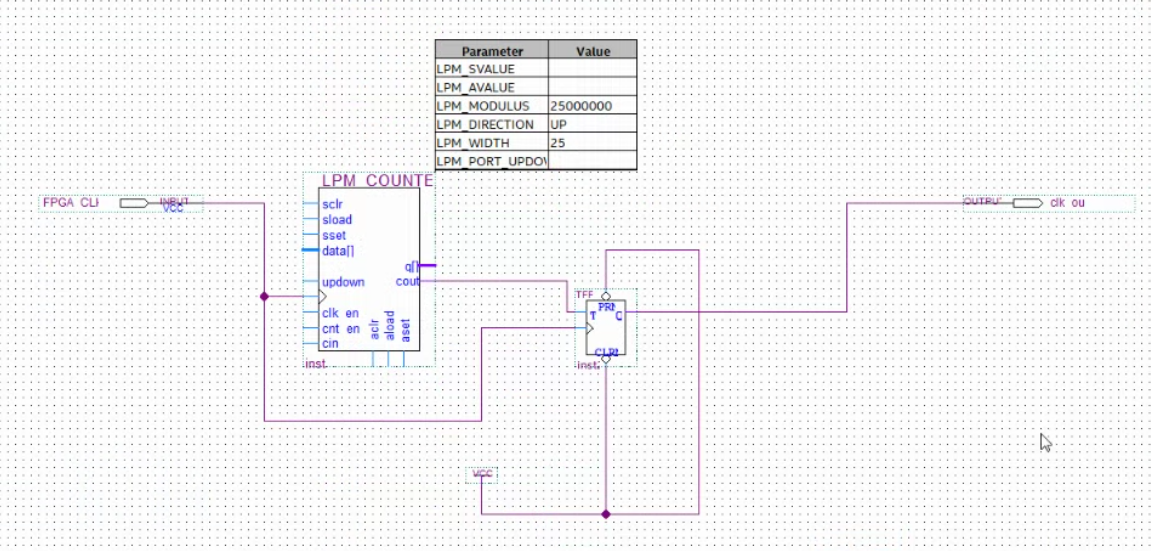
\includegraphics[width=1\columnwidth]{FIGURAS/cap_2/freq_1hz.png}
	\caption{Representação do bloco que gera um clock com frequência de 1Hz.}
        \label{fig:2.10}
\end{figure}


Com isto, obtem-se um clock com frequência de $1Hz$ na saída.

\section{Frequências acima de 1Hz}

Para as frequências acima de 1Hz, foi criado um divisor de clock autoral com precisão arbitrária. Foi escolhida uma precisão de $1\%$, mas era possível ter deixado mais preciso, dado que utilizaria-se um contador de mais bits.

Para conseguir a divisão precisa, inicialmente dividi-se o clock utilizando divisores, explicados na seção (2.2) para aproximar o clock da \emph{FPGA} com a frequência desejada, após isso utiliza-se o contador de 8 bits para dividir esta frequência reduzida e chegar a frequência desejada.

Segue abaixo, na Figura \ref{fig:2.11}, as divisões e contagens realizadas e suas margens de erro da desejada.

\begin{figure}[H]
	\centering
	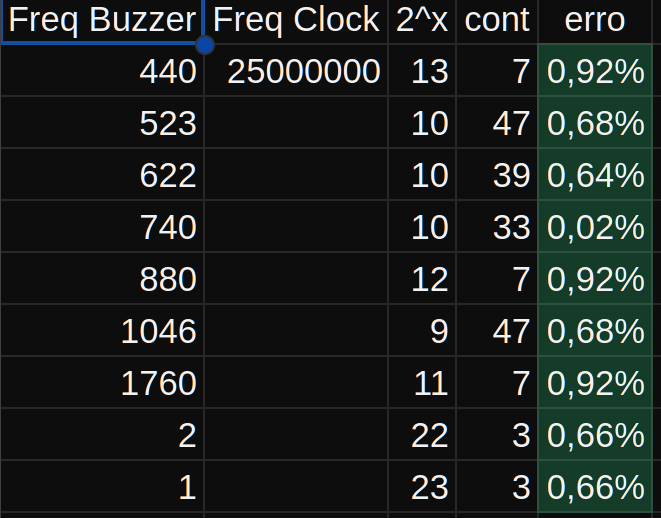
\includegraphics[width=1\columnwidth]{FIGURAS/cap_2/freq_tabela.png}
	\caption{Tabela de divisões e contagens para obtenção de cada frequência desejada.}
        \label{fig:2.11}
\end{figure}

%esse 2.5 tá okay?
Como pode-se ver na Figura \ref{fig:2.12}, para obtenção da frequência de $740Hz$ faz-se $2.5E7$ \emph{rising edges} dividido por $2^{10}$ pelos divisores, e novamente dividido por $33$ pelo contador de 8 bits.


\begin{figure}[H]
	\centering
	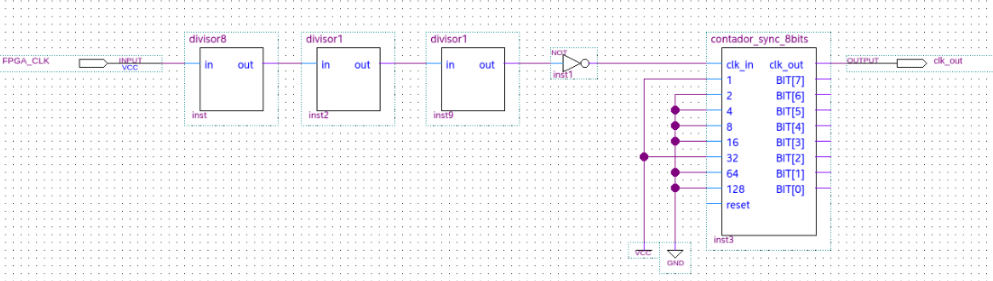
\includegraphics[width=1\columnwidth]{FIGURAS/cap_2/freq_740hz.png}
	\caption{Representação esquemática das divisões e contagens necessárias para obtenção de clock com frequência de 740Hz.}
        \label{fig:2.12}
\end{figure}



Neste caso em particular, obtem-se um erro de $0.02\%$, o menor que obteve-se em todas as frequências buscadas.

\section{Pulsos}

Outra técnica que foi utilizada foi transformar clocks em pulsos e vice-versa, como pode ser visto na Figura \ref{fig:2.13}.

\begin{figure}[H]
	\centering
	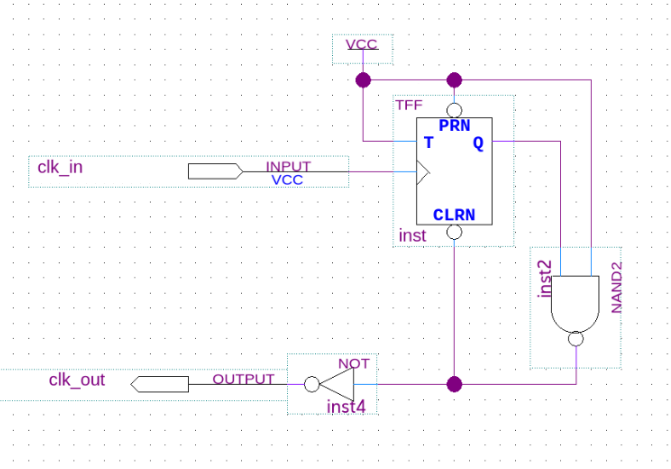
\includegraphics[width=1\columnwidth]{FIGURAS/cap_2/pulsos.png}
	\caption{Gerador de pulsos a partir de um clock de entrada.}
        \label{fig:2.13}
\end{figure}




Isso foi feito, pois um dos requerimentos do projeto foi utilizar um contador módulo 10 com frequência de clock de $1Hz$, que realizasse operações no estouro do clock.

Foi notado que não é preciso ligar o $V_{cc}$ na $NAND$, então não foi feita esta alteração, já que o design já havia sido terminado quando foi notado esta redundância.

\section{Debounce}

Foi notado que os botões da placa oscilam na sua transição de ligado para desligado à medida que o usuário aperta ou o solta.

Isso pode ocorrer pela instabilidade mecânica da mudança de estado entre ligado e desligado.

Para corrigir isto, foi criado um buffer com frequência de $110Hz$, que armazena os últimos 8 estados do botão. Se os 8 estiverem em nível lógico alto, o output resolve em nível lógico alto. Esse buffer pode ser visto na Figura \ref{fig:2.14}

\begin{figure}[H]
	\centering
	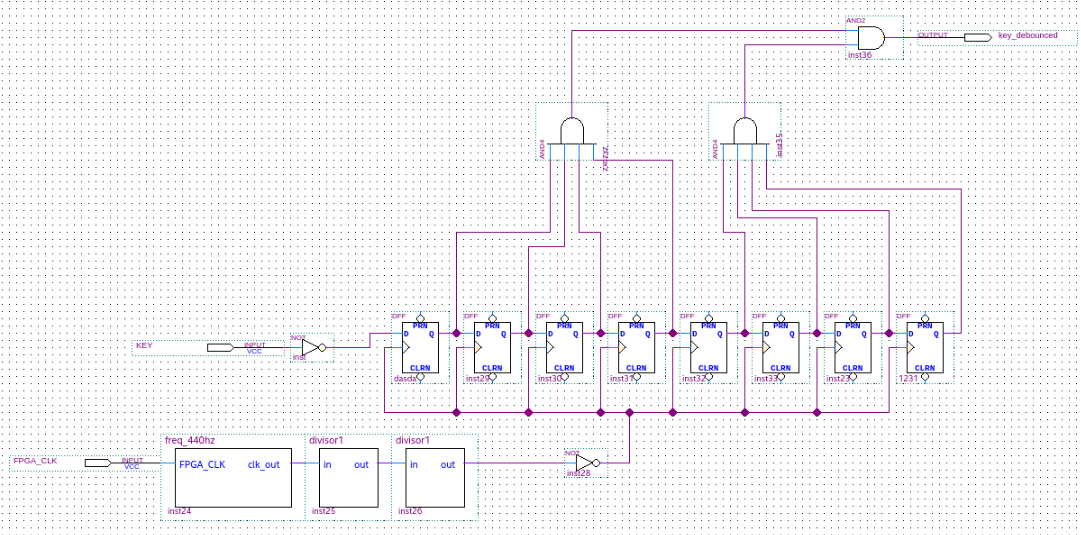
\includegraphics[width=1\columnwidth]{FIGURAS/cap_2/debounce.png}
	\caption{Representação debouncer para as teclas da placa.}
        \label{fig:2.14}
\end{figure}



Ou seja, para sair $1$ no output, precisa-se segurar o botão por $0.07$ segundos. Isto garante uma maior estabilidade no aperto do botão.

Menos buffers e uma frequência maior poderíam ter sido utilizados para obter uma boa estabilidade. Mas, testando empiricamente, este tempo de $0.07$ segundos não foi perceptível a ponto de ser problemático.





\section{Registradores}

Foi criado registradores de 4 bits e um banco de registradores. Esse banco tem 16 registradores de 4 bits, um para cada dígito da senha.

O banco de registradores fica responsável por: escolher qual é o dígito selecionado da senha no momento e informar quando o último dígito foi inserido corretamente.

Caso haja algum erro na inserção da senha, ela é resetada de volta para o primeiro dígito.

\subsection{Registrador de 4 bits}

Foi utilizados estes registradores, que podem ser vistos na Figura \ref{fig:2.15}, para armazenar os hexadecimais da senha.


\begin{figure}[H]
	\centering
	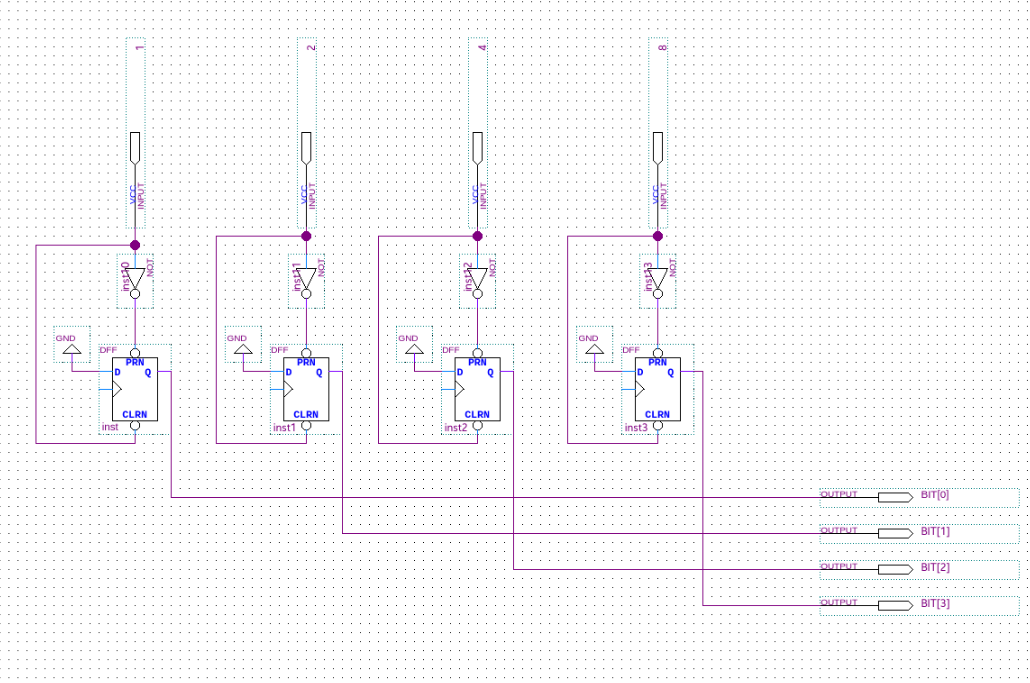
\includegraphics[width=1\columnwidth]{FIGURAS/cap_2/registrador.png}
	\caption{Registrador de 4 bits.}
        \label{fig:2.15}
\end{figure}

Os inputs escolhidos pelo desenvolvedor decidirão o estado do registrador, ou seja, seus outputs.

\subsection{Banco de registradores}

Tem-se um contador de 8 bits com módulo 16 na entrada. Este dirá quando o último dígito foi inserido, ou seja, quando seu carry out subir o nível lógico. Ele também dirá em qual digito está atualmente, ou seja, qual registrador deve ser selecionado atualmente.

Quando houver um clock in no contador, altera-se o registrador que dará o valor de saída para o seguinte. E se o hexadecimal da senha for o incorreto, reseta-se o contador, ou seja, volta-se a utilizar o primeiro registrador como o output. Uma parte desse sistema esta na Figura \ref{fig:2.16}.

\begin{figure}[H]
	\centering
	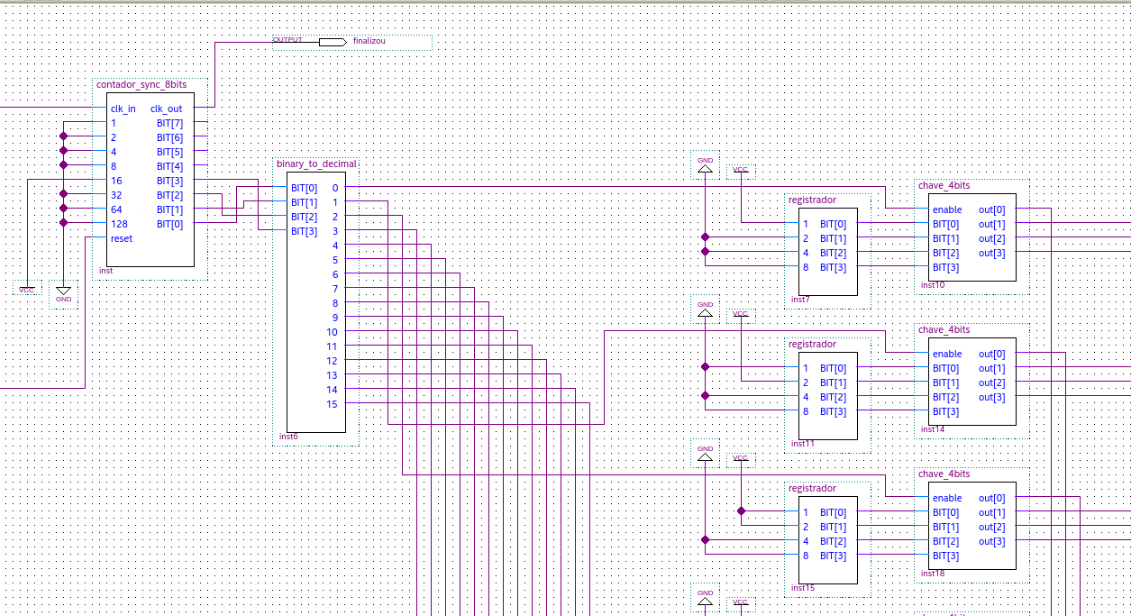
\includegraphics[width=1\columnwidth]{FIGURAS/cap_2/banco_registradores.png}
	\caption{Parte do banco de registradores.}
        \label{fig:2.16}
\end{figure}

Nos registradores foi escolhido uma senha fixa do sistema. Para este projeto foi determinado que a senha seria $[1, 2, 3, 4, 5, 6, 7, 8, 9, 10, 11, 12, 13, 14, 15, 0]$. 

Quando concluída corretamente, o dígito da senha retorna para o inicial. Isso não será um problema, já que, no projeto, para-se a contagem quando este contador estourar.


\section{Prioridade}

Ao apertar um botão enquanto o buzzer estava tocando o som de uma frequência, foi notado que estava havendo uma interferência entre a frequência do botão anterior e a do botão atual. Para resolver isso, foi feito um sistema de prioridades de frequências, que faz com que apenas a frequência do ultimo botão apertado seja enviada.

Para isso, foram utilizados 6 entradas e 6 flip-flops do tipo \emph{t} que recebem pela porta \emph{PRN} um pulso gerado quando alguma frequência será enviada, seja por apertar um botão ou ao comparar os valores inseridos pelo usuário. Além disso, os flip-flops de cada entrada foram conectados à uma porta lógica OR com 5 entradas, que recebe o pulso das outras 5 entradas. Portanto, se a saída do primeiro flip-flop é 1 e algum outro botão for apertado, o pulso desse botão irá para a porta \emph{CLRN} do flip-flop e a saída passará a ser 0, enquanto a saída do flip-flop desse botão apertado passará a ser 1.

A representação desses flip-flops pode ser vista na Figura \ref{fig:2.17} abaixo.

\begin{figure}[H]
	\centering
	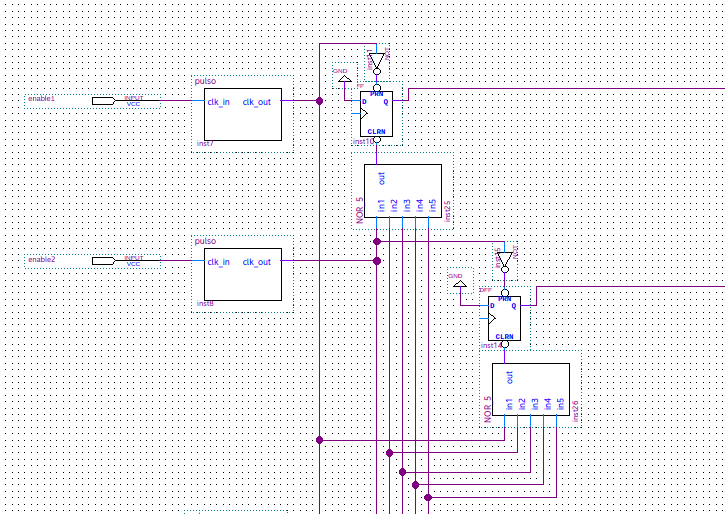
\includegraphics[width=1\columnwidth]{FIGURAS/cap_2/prioridade_enable.png}
	\caption{Parte do sistema de prioridades.}
        \label{fig:2.17}
\end{figure}

As saídas dos flip-flops estão conectadas a uma porta lógica AND, em que uma entrada é o \emph{enable}, que no caso são as saídas dos flip-flops, e a outra entrada é a frequência. Portanto, enquanto a saída de um flip-flop for 1, a frequência continuará sendo enviada. A partir do momento em que outro botão for apertado, o \emph{enable} da frequência anterior passará a ser 0 e não permitirá a passagem da frequência. Enquanto isso, o \emph{enable} do botão mais recente será 1 e permitirá a passagem da sua respectiva frequência.

As saídas das portas lógicas \emph{AND} serão enviadas para uma porta lógica \emph{OR} com 6 entradas que mandará a frequência mais recente para o buzzer. Essa parte do circuito pode ser vista na Figura \ref{fig:2.18} abaixo.

\begin{figure}[H]
	\centering
	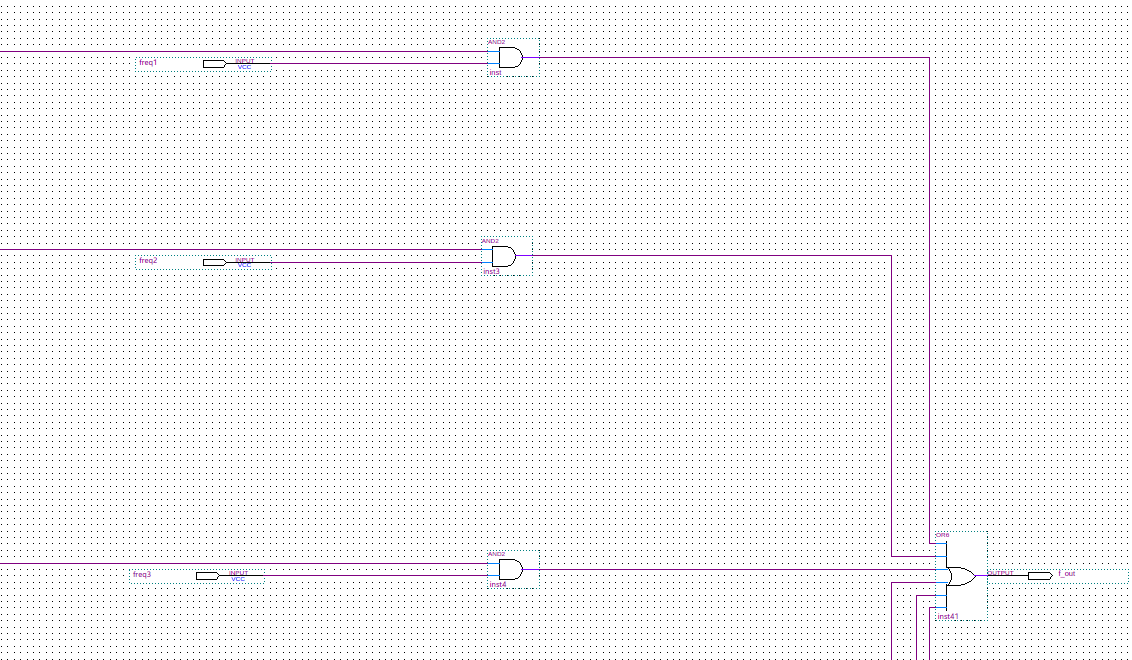
\includegraphics[width=1\columnwidth]{FIGURAS/cap_2/prioridade_f.png}
	\caption{Parte do sistema de prioridades.}
        \label{fig:2.18}
\end{figure}



\section{Comparador}

Para ser feita a comparação da entrada do usuário com a senha escolhida, foram utilizadas quatro portas lógicas XOR e uma NOR. As portas lógicas XOR recebem em uma entrada os bits inseridos pelo usuário e na outra os bits do registrador que armazena a senha. Portanto, se os bits forem iguais as saídas das portas lógicas XOR serão 0. Essas saídas são as entradas da porta lógica OR. Com isso, se todas as entradas forem 0, a saída será 1, o que significa que todos os bits são iguais. Esse comparador pode ser visto na Figura \ref{fig:2.19}.

\begin{figure}[H]
	\centering
	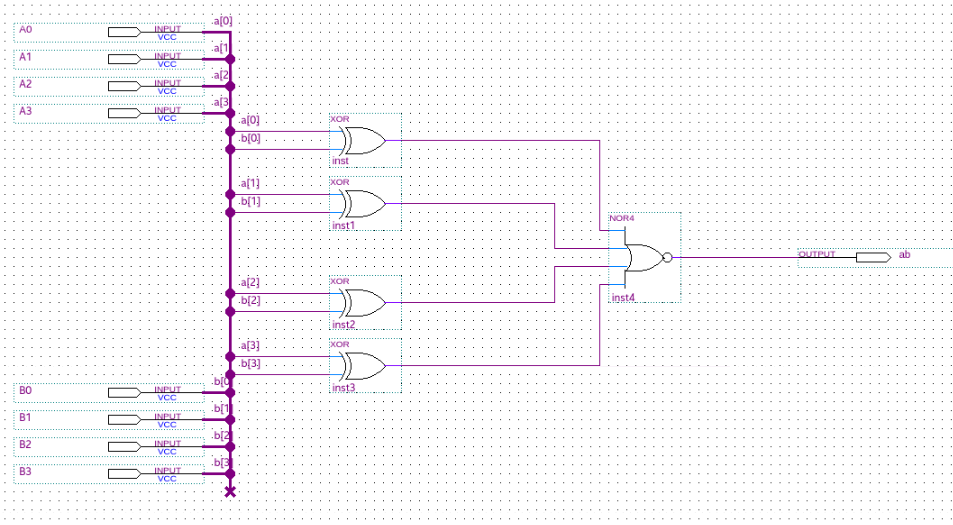
\includegraphics[width=1\columnwidth]{FIGURAS/cap_2/comparador.png}
	\caption{Representação esquemática do comparador.}
        \label{fig:2.19}
\end{figure}

\section{LED e Buzzers}

Foi criada uma função que recebe o input do botão, acende um LED e emite uma frequência, que será definida pela entrada. Uma parte dessa função pode ser vista na Figura \ref{fig:2.20}.

\begin{figure}[H]
	\centering
	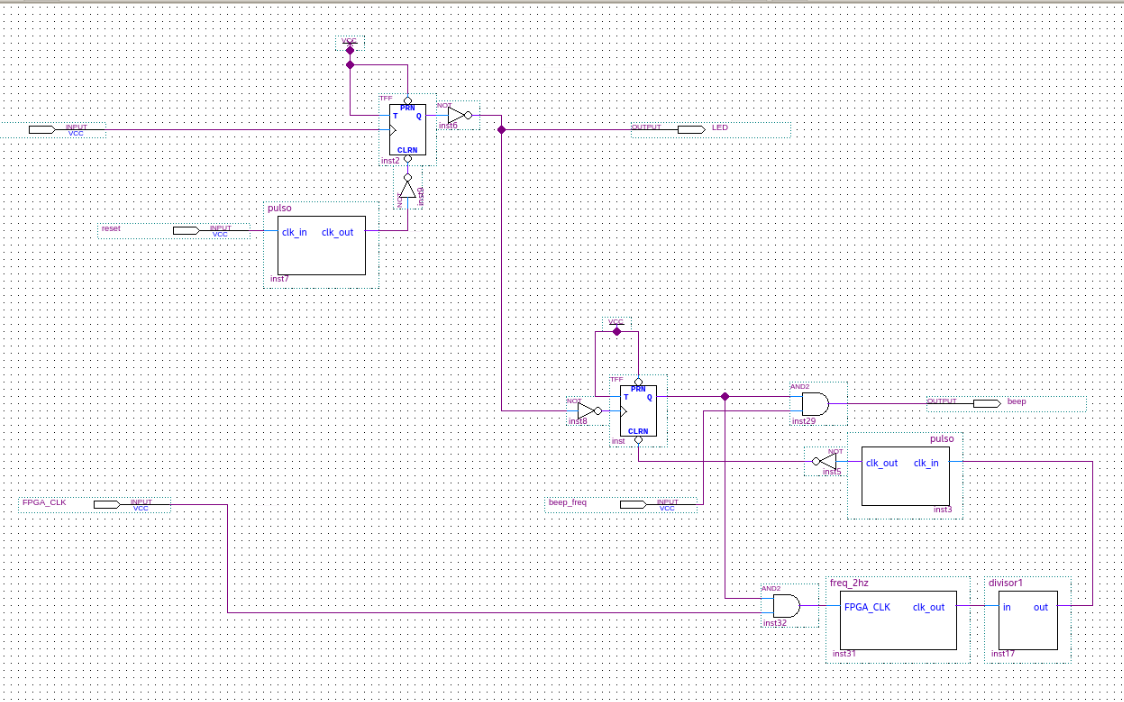
\includegraphics[width=1\columnwidth]{FIGURAS/cap_2/led_buzzer.png}
	\caption{Parte do banco de registradores.}
        \label{fig:2.20}
\end{figure}

A ideia é: o input do botão entra direto para o LED e desce para inicializar um flip-flop, o alterando de nível lógico baixo para alto.

Quando este flip-flop ativa, ele permite a passagem de uma frequência de entrada para o buzzer, e ao mesmo tempo, permite a passagem da frequência do FPGA para um divisor de frequência que tem clock de saída de $2Hz$. Esse clock de saída será divido por 2 para obtermos $1Hz$, que é o tempo que quer-se que o buzzer emite som.

Quando esta frequência atinge seu primeiro ponto de nível lógico alto, ela entra em uma função pulso, que dará clear no flip-flop para dar-se mute no buzzer novamente.

E isso só se ativará novamente no próximo nível lógico alto do botão de entrada.

Essencialmente, foi criado um timer de 1 segundo que se inicia assim que o buzzer liga. Ele foi utilizado para dar mute no buzzer.




\section{Display de sete segmentos}

%duas figuras 21?
Os 4 bits de saída do contador mod10 foram utilizadas como entrada para o bloco do display de 7 segmentos, como visto na Figura \ref{fig:2.21}. Ele utiliza um conjunto de portas lógicas para considerar quais segmentos do display deverão ser ligados. Isso ocorre com o objetivo de representar o número decimal no visor, para que o usuário possa acompanhar quanto tempo lhe resta para informar ao hardware o próximo valor de 4 bits da senha armazenada.

%Figura 21, dos 4 bits com seus nots
\begin{figure}[H]
	\centering
	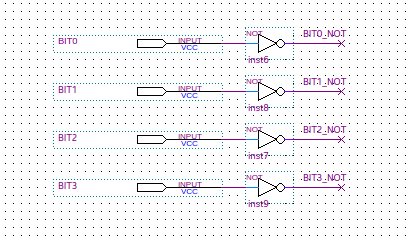
\includegraphics[width=1\columnwidth]{FIGURAS/cap_2/EntradasBITS.png}
	\caption{Entradas do display de sete segmentos.}
        \label{fig:2.21}
\end{figure}


Para que um segmento do display se acenda no momento correto, é necessário que ele receba um sinal sempre que o contador chegar a um valor, cuja representação em decimal se utilize daquele segmento. Por existir a possibilidade de múltiplos números se utilizarem do mesmo segmento, foram implementadas algumas portas lógicas NOR. Um exemplo dessas portas esta na Figura \ref{fig:2.22}. As portas lógicas NOR foram utilizadas em detrimento de portas OR devido a característica da placa de "ligada" em nível lógico baixo.

%Figura 22, com um exmplo de um NOR
\begin{figure}[H]
	\centering
	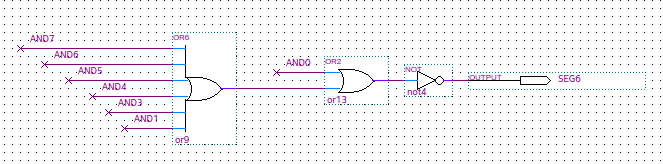
\includegraphics[width=1\columnwidth]{FIGURAS/cap_2/ExemploNOR.png}
	\caption{Exemplo de uma porta lógica NOR que tem saída no segmento 0 do display.}
        \label{fig:2.22}
\end{figure}


Elas passarão o sinal para o segmento, caso o contador chegue a qualquer um dos valores que utilize aquele segmento. Este sinal recebido pela porta-lógica NOR advém das saídas de portas-lógicas AND, que tem como papel, definir quais devem ser os valores do contador que acenderão um determinado segmento. Um exemplo de uma porta lógica AND está na Figura \ref{fig:2.23}.

%Figura 23, exemplo de uma AND
\begin{figure}[H]
	\centering
	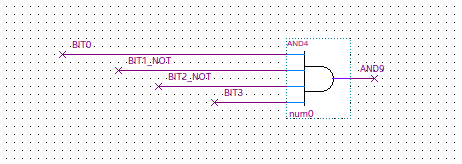
\includegraphics[width=1\columnwidth]{FIGURAS/cap_2/ExemploAND.png}
	\caption{Exemplo de uma AND que representa a seleção do número em decimal.}
        \label{fig:2.23}
\end{figure}